\documentclass[conference]{IEEEtran}
\usepackage{graphicx}
\usepackage{booktabs}
\usepackage[hidelinks]{hyperref}

\begin{document}

\title{A Multi-Region, Event-Labeled Sensor-Network Dataset\\
for Spatial Event Localization}

\author{\IEEEauthorblockN{[Author 1], [Author 2], [Author 3], [Author 4]}
\IEEEauthorblockA{Ottawa University, Surprise, AZ, USA \\
[contact email]}}

\maketitle

\begin{abstract}
Spatial event localization asks a model to find \emph{where} an
environmental event happened using only the time series of a fixed sensor
network. Training and evaluating such models requires datasets that pair
sensor measurements with independently documented ground-truth events,
including each event's time, location, extent, and the reliability of that
information. We present an openly packaged dataset built for this task:
hourly air-quality and meteorological measurements from 516 stations across
five US Southwest states and six European cities (2022 through mid-2026),
paired with $\sim$1,700 wildfire and dust-storm events taken exclusively
from authoritative government and satellite records. Events carry quality
tiers, official area geometries, and, for fires, the registry's ignition
point and size at discovery.
\end{abstract}

\section{Motivation}
Sensor networks record what the atmosphere does, but rarely \emph{why}.
The missing piece for localization research is ground truth:
a record of real events whose time, place, and extent are known
independently of the sensors. Hand-labeling events from the measurements
themselves is circular---a model evaluated on such labels is evaluated on
another model's opinion. We therefore built a dataset in which every event
comes from an official registry, every claim about an event can be traced
to a public source, and the known imprecision of each source is encoded in
the data rather than hidden.

\section{Dataset Construction}
\textbf{Sensors.} We compiled the list of regulatory air-quality stations
in Arizona, California, Nevada, New Mexico, and Utah from the US EPA Air
Quality System bulk archive, and in Berlin, Munich, Paris, Rome, Lisbon,
and Stockholm from the European Environment Agency's e-Reporting database.
Per station and hour the dataset carries PM2.5, PM10, NO$_2$, SO$_2$, CO,
and O$_3$; not every station measures every pollutant
(Table~\ref{tab:regions}). Meteorological variables (temperature, surface
pressure, precipitation, wind speed and direction) are spatially
interpolated from the native ERA5 reanalysis grid to each station location
and joined by UTC timestamp, giving near-complete weather coverage at
every station.

\textbf{Events.} We matched the sensor regions to real-world events
obtained from the NIFC WFIGS interagency fire registry (US wildfires,
including mapped perimeters and ignition records), the NOAA Storm Events
database (US dust storms), and NASA FIRMS/VIIRS satellite detections
(European fires). We categorized events as wildfires, dust storms, and
other recurring events, and assigned each a quality tier: tier~1, place
and time precise; tier~2, time precise but location zone-level
($\pm$15--25\,km); tier~3, predictable or recurring patterns.

\textbf{Quality control.} Every fire with a mapped perimeter is
cross-checked automatically: the ignition point must fall inside the
perimeter, and the registry's reported acreage must agree with the area of
the GIS polygon. Verdicts are stored per event as filterable columns.

\textbf{Code.} The full pipeline---data download, conversion, weather
join, event matching, geometry audits, and every figure in this
paper---is available at
\url{https://github.com/NilsHRose/wno-event-dataset}.

\begin{table}[t]
\caption{Dataset summary by region (2022 -- June 2026).}
\label{tab:regions}
\centering
\small
\begin{tabular}{lrrrr}
\toprule
Region & Sensors & Fires & Dust & Other \\
\midrule
Arizona & 83 & 267 & 67 & 117 \\
California & 244 & 209 & 22 & 83 \\
Nevada & 36 & 122 & 17 & 35 \\
New Mexico & 30 & 177 & 18 & 8 \\
Utah & 35 & 100 & 2 & 3 \\
Berlin & 14 & 8 & 0 & 25 \\
Lisbon & 15 & 19 & 0 & 23 \\
Munich & 5 & 1 & 0 & 31 \\
Paris & 31 & 7 & 0 & 24 \\
Rome & 13 & 63 & 0 & 22 \\
Stockholm & 10 & 7 & 0 & 21 \\
\midrule
\textbf{Total} & \textbf{516} & \textbf{980} & \textbf{126} & \textbf{392} \\
\bottomrule
\end{tabular}
\end{table}

\begin{figure*}[t]
\centering
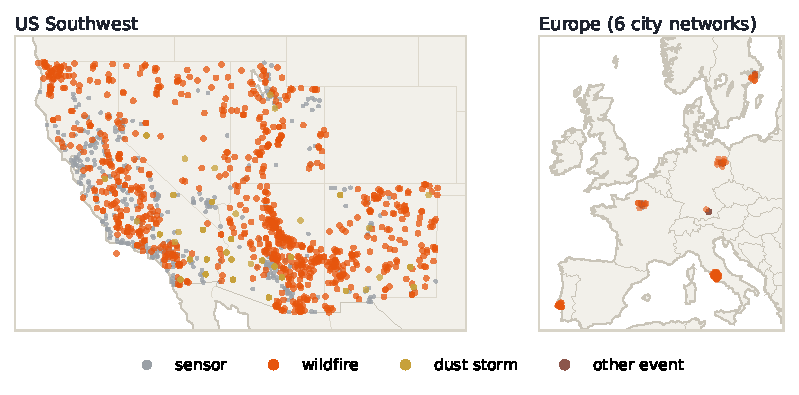
\includegraphics[width=0.78\textwidth]{figs/fig_map.pdf}
\caption{Sensor and event distribution. Gray: air-quality stations.
Orange: wildfires; tan: dust storms; brown: other events. Left: five US
Southwest states; right: the six European city networks.}
\label{fig:map}
\end{figure*}

\section{Observations}
Fig.~\ref{fig:temporal} shows the dataset around one event, the Juniper
Fire (Arizona, July 2, 2025), for the three nearest stations with data.
We observed that the event dominates the particulate channels: PM10 rises
from a baseline below 50\,\textmu g/m$^3$ to nearly
1,000\,\textmu g/m$^3$ at stations 43--56\,km from the ignition point,
and PM2.5 shows the same rise where it is measured. Wind speed, by
contrast, keeps its ordinary diurnal rhythm---features differ sharply in
how strongly an event affects them, which is exactly the structure a
localization model must exploit. Fig.~\ref{fig:spatial} shows the same
event spatially: the 48-hour PM10 maximum per station forms a coherent
footprint around the ignition point (star), while remote stations stay at
baseline.

We also observed the main limitations. Zone-based reports (dust storms)
carry no exact location---the coordinate is the forecast-zone centroid.
Therefore we encode location quality explicitly as the tier system and
attach the official zone polygon instead of pretending point precision.
Perimeters are mapped only for a subset of fires (final extent only, not
daily spread), stations report different pollutant subsets, and
particulate signatures of fires and dust storms can resemble each other,
so event type must come from the registry, not the signal alone.

\begin{figure}[!t]
\centering
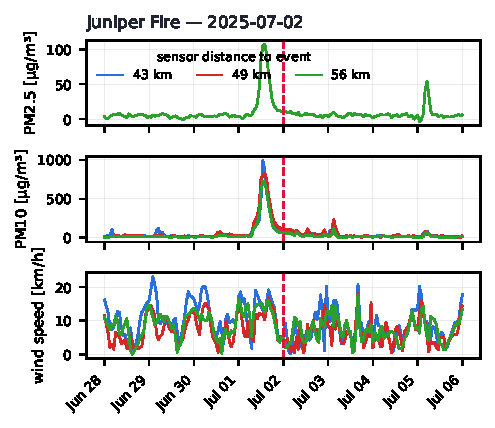
\includegraphics[width=0.93\columnwidth]{figs/fig_temporal.pdf}
\caption{Temporal view: three stations (by distance to the event),
three features, $\pm$96\,h around the Juniper Fire (dashed line).}
\label{fig:temporal}
\end{figure}

\begin{figure}[!t]
\centering
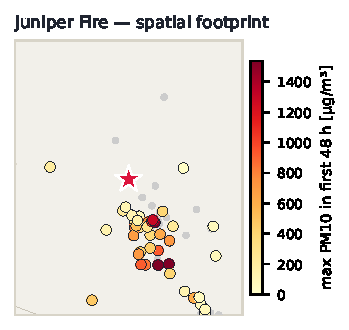
\includegraphics[width=0.84\columnwidth]{figs/fig_spatial.pdf}
\caption{Spatial view of the same event: per-station PM10 maximum in the
first 48\,h; the star marks the event location.}
\label{fig:spatial}
\end{figure}

\section{Discussion and Intended Use}
The dataset is built to train and evaluate spatial localization models:
given the multivariate sensor field over a time window, predict where the
source is. The event tables provide the targets (point, and area where
available); the tier system separates a strict tier-1 benchmark from the full set; and the polygons support evaluating
``prediction inside the affected area'' rather than point distance. We propose to use the data with distance-weighted baselines, graph
neural networks over the station graph, sequence models, and our upcoming
wavelet-neural-operator approach (WNO-Loc), which treats the station
field as a function and localizes sources from its multiscale structure.

\vspace{2pt}{\footnotesize\noindent\textit{Acknowledgment ---} Code and language editing were assisted by an AI system (Anthropic Claude); all data and statements were verified by the authors.\par}

\end{document}
